\documentclass[../../main.tex]{subfiles}
\graphicspath{{\subfix{../../diagrams/}}}
\usepackage{lipsum}  
\usepackage{float}

\begin{document}
\begin{figure}[ht!]
\caption{Client module class diagram.}
\vspace{10mm}
\centering
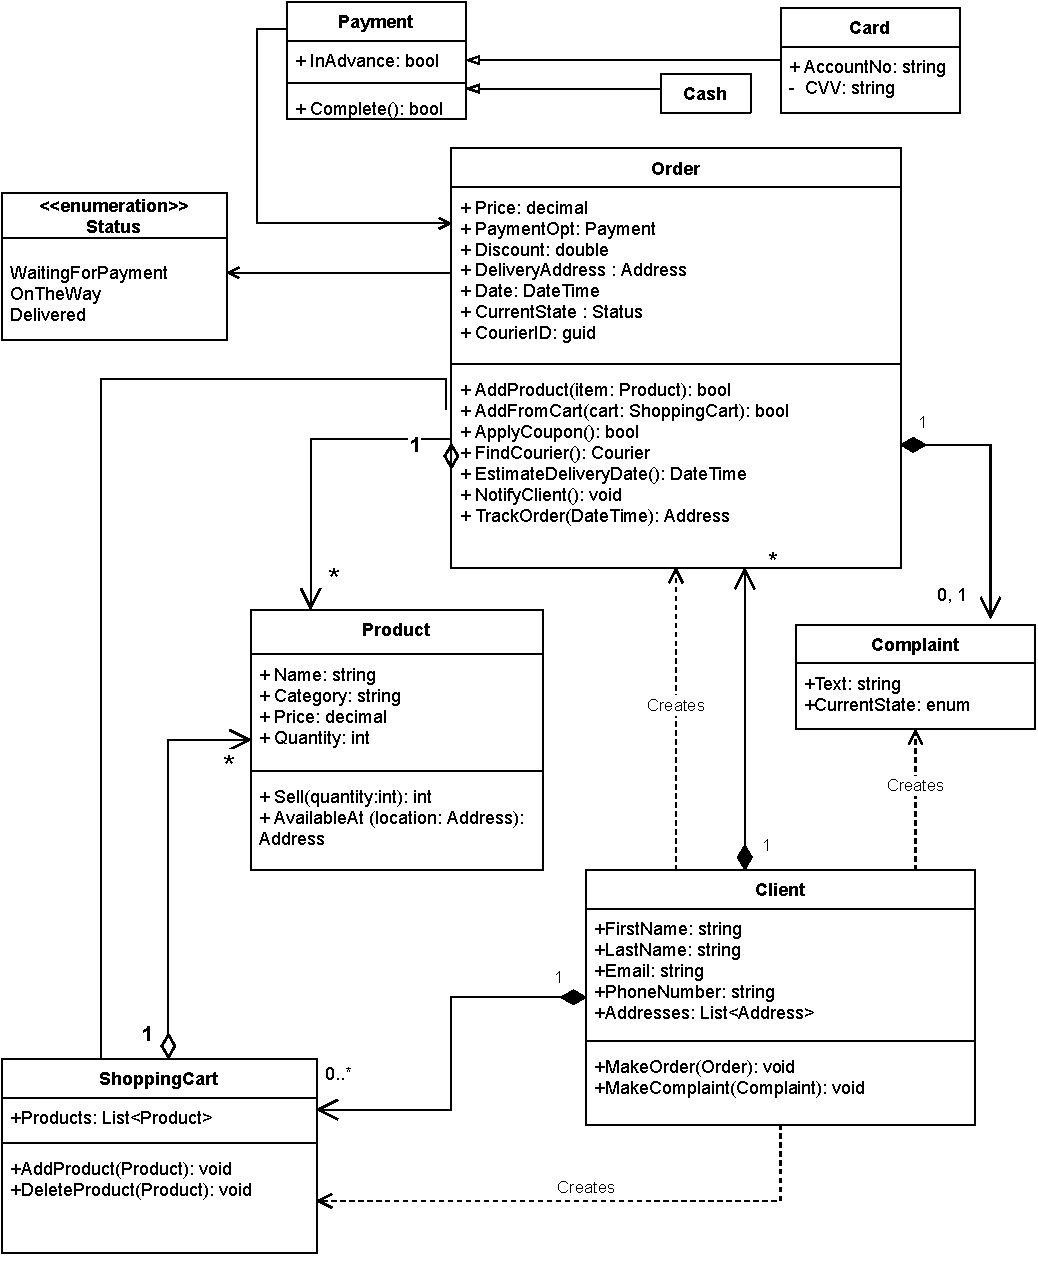
\includegraphics[width=1\textwidth]
{class-diagrams/client-class-diagram.pdf}
\end{figure}


\subsubsection{Client}
This class represents a customer in our system. Required data about the client is collected during the registration, where an instance of this class is created. The class consists of necessary fields for delivering the order and contacting the client. This class also has methods representing their certain activities (\textbf{MakeOrder}, \textbf{MakeComplaint}). A client can have any number of orders (type \textbf{Order}) and can, but is not required to, have a \textbf{ShoppingCart} for items.

\subsubsection{Order}
This class describes a shopping order in the context of being created, customized, then monitored by a client.
A list of products is represented by one of the class' public fields. When a client wants to buy something immediately (\textbf{AddProduct} method) or after finishing his \textbf{ShoppingCart} (\textbf{AddFromCart} method) the new estimated \textbf{Price} is calculated. Once the client proceeds to payment, the \textbf{PaymentOpt} is chosen and other fields are set as well. The \textbf{CurrentState} changes accordingly to whether or not the client has paid, if the deliverer has gone to deliver the package and if the client received it.

Methods that are used when a client wants to monitor the package after finalizing the order are \textbf{EstimateDeliveryData}, \textbf{NotifyClient} and \textbf{TrackOrder}.

\subsubsection{Product}
This class represents a product, mainly from a client's perspective, as an element in their shopping cart or order. It has a \textbf{Price}, can be searched by \textbf{Category} and the \textbf{Quantity} can be specified. The \textbf{Quantity} sold can be recorded by the Shop through \textbf{Sell()} and checked for availability with \textbf{AvailableAt()} methods.

\subsubsection{ShoppingCart}
This class describes a shopping cart, to which products can be added to and removed freely. Once the cart is confirmed, the items are all added to the actual order's list of products that will be shipped to the client later on.

\end{document}
